%%%%%%%%%%%%%%%%%%%%%%%%%%%%%%%%%%%%%%%%%%%%
% https://github.com/martinhelso/uioposter %
%%%%%%%%%%%%%%%%%%%%%%%%%%%%%%%%%%%%%%%%%%%%
% Class options                            %
%%%%%%%%%%%%%%%%%%%%%%%%%%%%%%%%%%%%%%%%%%%%
% Orientation:                             %
% portrait (default), landscape            %
%                                          %
% Paper size:                              %
% a0paper (default), a1paper, a2paper,     %
% a3paper, a4paper, a5paper, a6paper       %
%                                          %
% Language:                                %
% english (default), norsk                 %
%%%%%%%%%%%%%%%%%%%%%%%%%%%%%%%%%%%%%%%%%%%%
\documentclass{uioposter}

\usepackage[absolute, overlay]{textpos}            % Figure placement
\setlength{\TPHorizModule}{\paperwidth}
\setlength{\TPVertModule}{\paperheight}

% Wrap figure
\usepackage{wrapfig}

% Table rules
\usepackage{booktabs}

% Bibliography
\usepackage{ifplatform}
\usepackage[style=apa,sortcites=true,sorting=nyt,backend=biber, useprefix=false]{biblatex}
\ifwindows
    \addbibresource{M:\\pc\\Dokumenter\\MSc\\Thesis\\Bibliography\\Master.bib}
\else
    \addbibresource{~/uio/pc/Dokumenter/MSc/Thesis/Bibliography/Master.bib}
\fi


\title{School Climate and Youth's Financial Literacy Outcomes}
\author
{%
    Candidate: Tony Tan%\inst{1}
    \and
    Supervisors: Prof Ronny Scherer%\inst{1}
    \and
    Dr Chia-Wen Chen%\inst{1}
}
%% Optional:
% \institute
% {
%     \inst{1} Centre for Educational Measurement
%     \and
%     \inst{2} Det utdanningsvitenskapelige fakultet
% }
% Or:
\institute{Centre for Educational Measurement, Faculty of Educational Sciences, University of Oslo}


%% Remove footline:
%\setbeamertemplate{footline}{}


\begin{document}

\begin{frame}

\begin{columns}[onlytextwidth]

% Begin left column
\begin{column}{0.5\textwidth - 1.5cm}

    \begin{block}{Introduction}
        \begin{wrapfigure}{r}{0.5\linewidth}
            \centering
            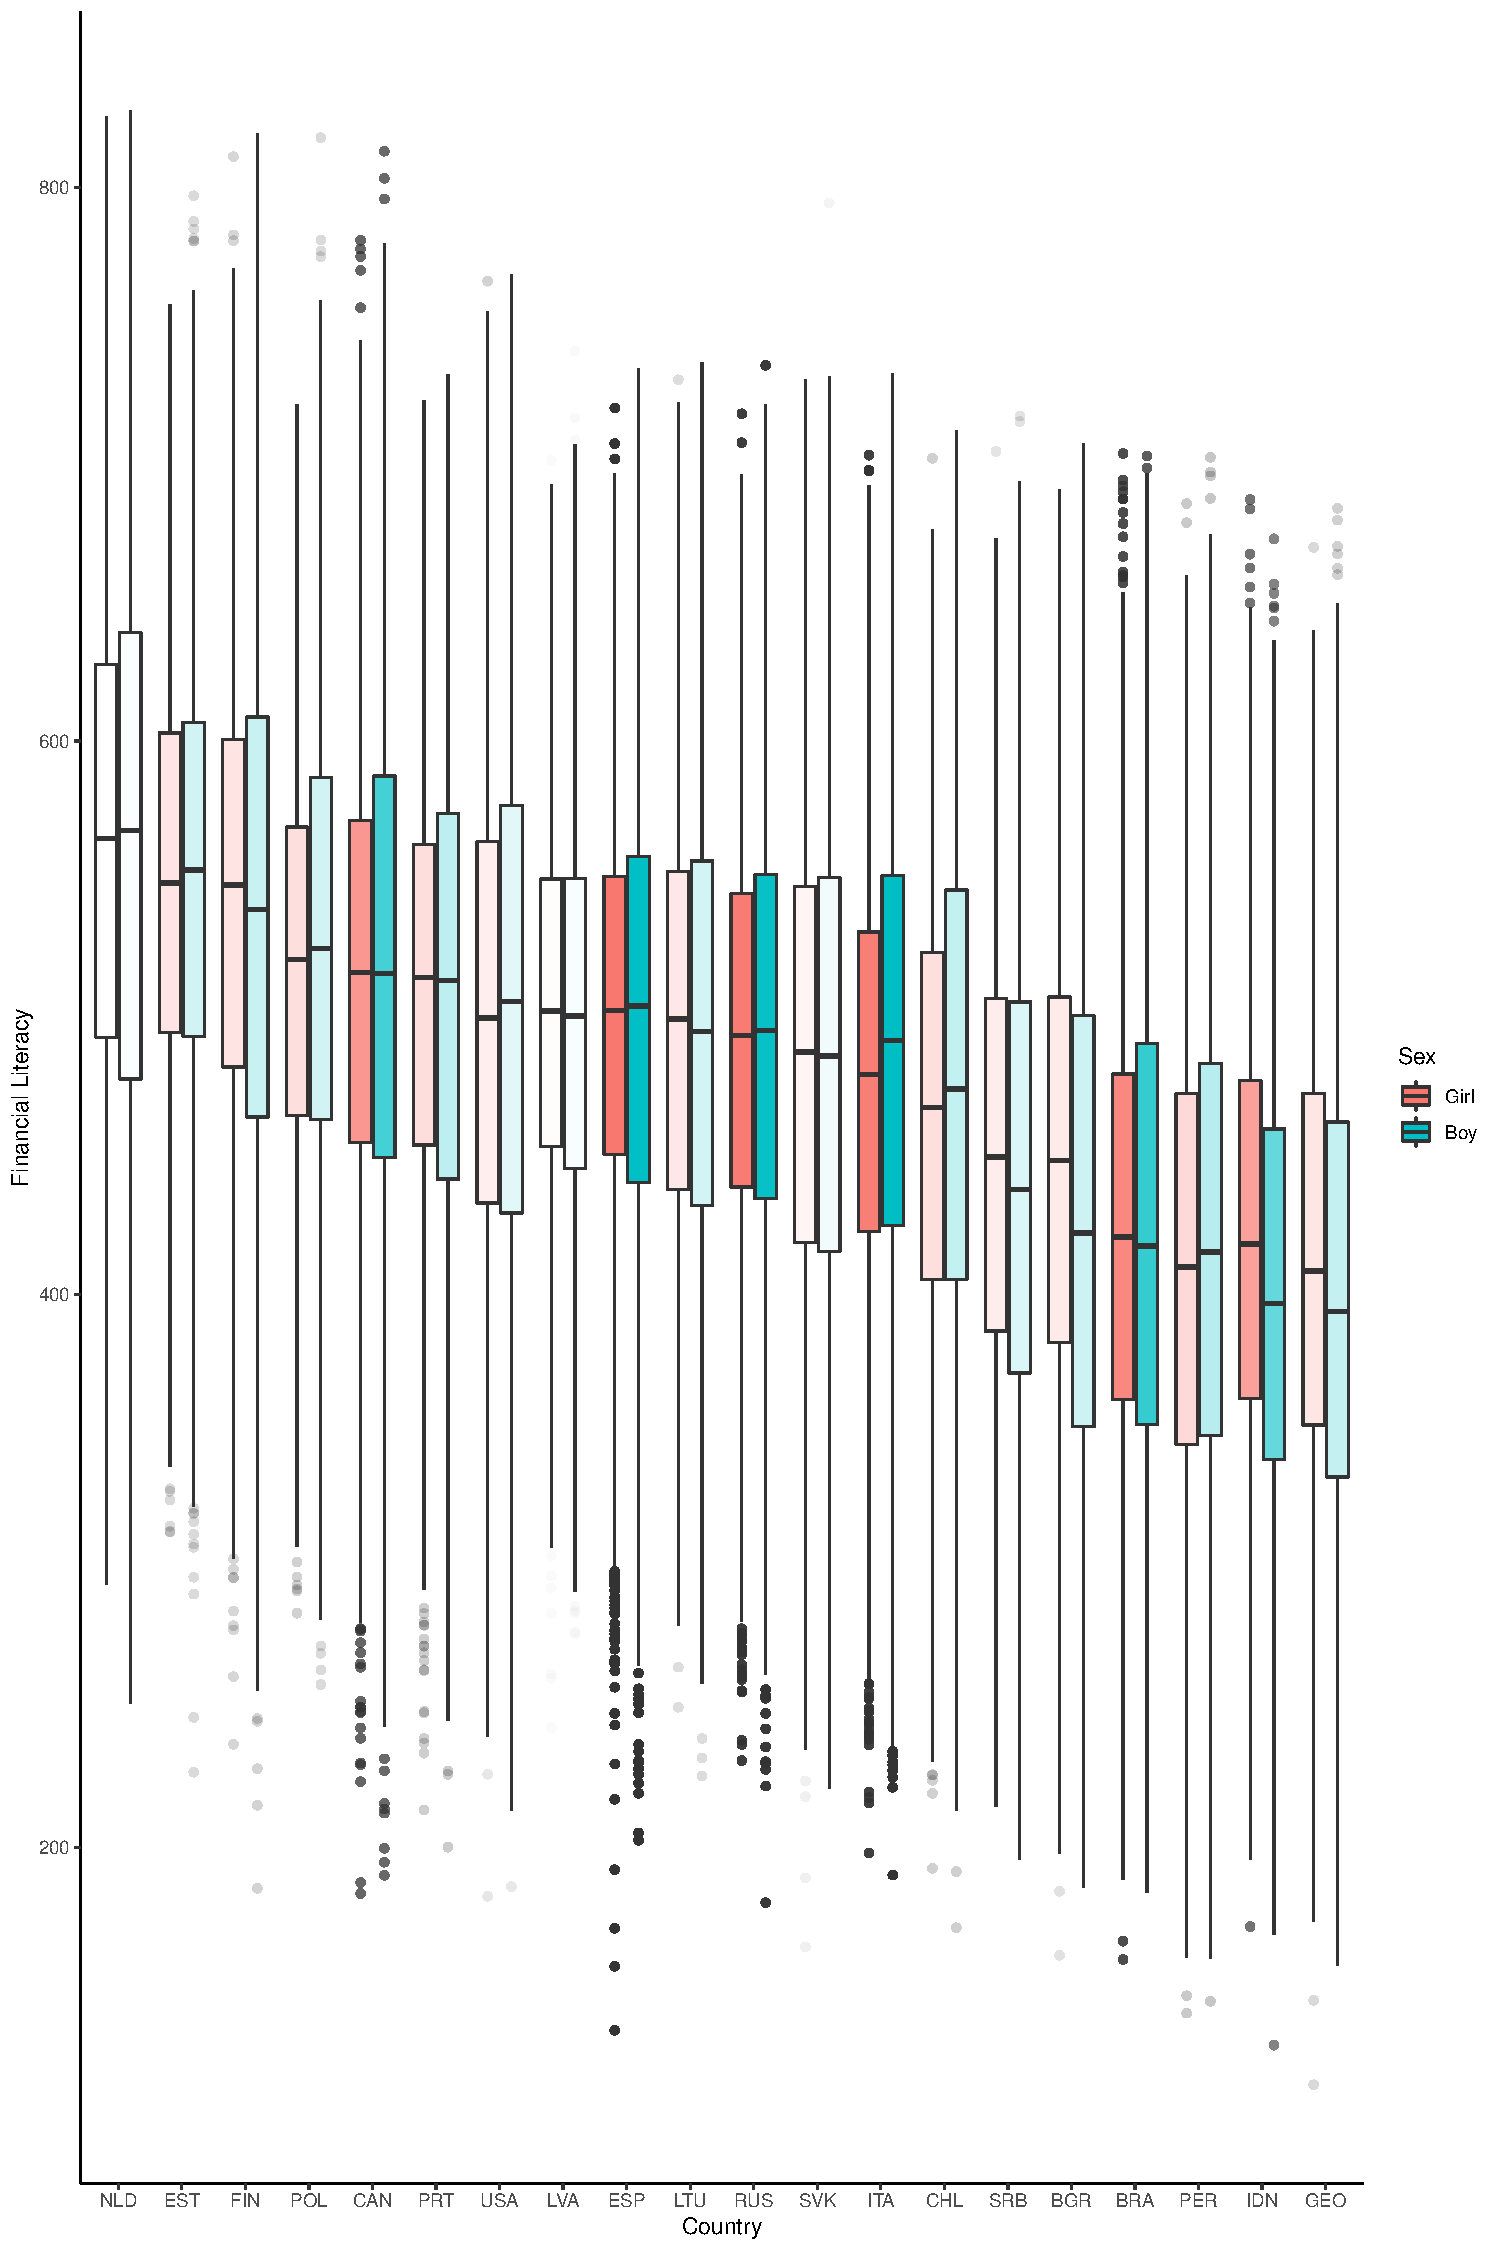
\includegraphics[width=0.5\textwidth]{../Figures/distribution.pdf}
        \end{wrapfigure}
        Repeated economic crises in recent memory has exposed the cost of financial \emph{illiteracy}. Redress schemes are shown to be most effective if introduced early in life \parencite{lusardi:2014}. OECD's triennial Programme for International Student Assessment (PISA) has been tracking 15-year-olds' financial literacy levels since 2012 with the latest 2018 results showing sizeable differences across the globe. This study attempts to identify school climate variables that covary strongly with youth's financial literacy outcomes for the purpose of lending support to school leaders and policy makers in their evidence-based decision making.
    \end{block}

    \begin{block}{Research Questions}
        \begin{enumerate}
            \item[RQ1:] To what extent can the variation in students' financial literacy outcomes be accounted for by each of the school climate variables?
            \item[RQ2:] In particular, how do cognitive and affective pathways interact during classroom financial literacy interventions?
        \end{enumerate}
    \end{block}

    % Begin{exampleblock}{Black}
    %      Use an \structure{gray text}
    % \end{exampleblock}

    % \begin{alertblock}{How do you make it pop?}
    %     Use an \alert{alertblock}!
    % \end{alertblock}

    \begin{block}{School Climate Variables \parencite{wang:2016}}
        % Table generated by Excel2LaTeX from sheet 'Sheet1'
\begin{table}
  \centering
    \begin{tabular}{clc}
    \toprule
    Aspect of      & \multicolumn{1}{c}{Operationalisation} & Variable \\
    school climate & \multicolumn{1}{c}{from 2018 PISA data files} & label \\
    \midrule
    Academic & 931: Financial education in & \texttt{FLSCHOOL} \\
             & school lessons              & \\
    Community & 932: Parental involvement in & \texttt{FLFAMILY} \\
              & matters of Financial Literacy & \\
    Safety & 916: Stdent's experience of & \texttt{NOBULLY} \\
           & being bullied (reverse coding) & \\
    Institutional & 188: Shortage of educational & \texttt{EDUSHORT} \\
    environment   & material                     & \\
    \bottomrule
    \end{tabular}
\end{table}

    \end{block}

\end{column}
% End left column

% Begin right column
\begin{column}{0.5\textwidth - 1.5cm}

    \begin{block}{Model and Result}
        \begin{figure}
            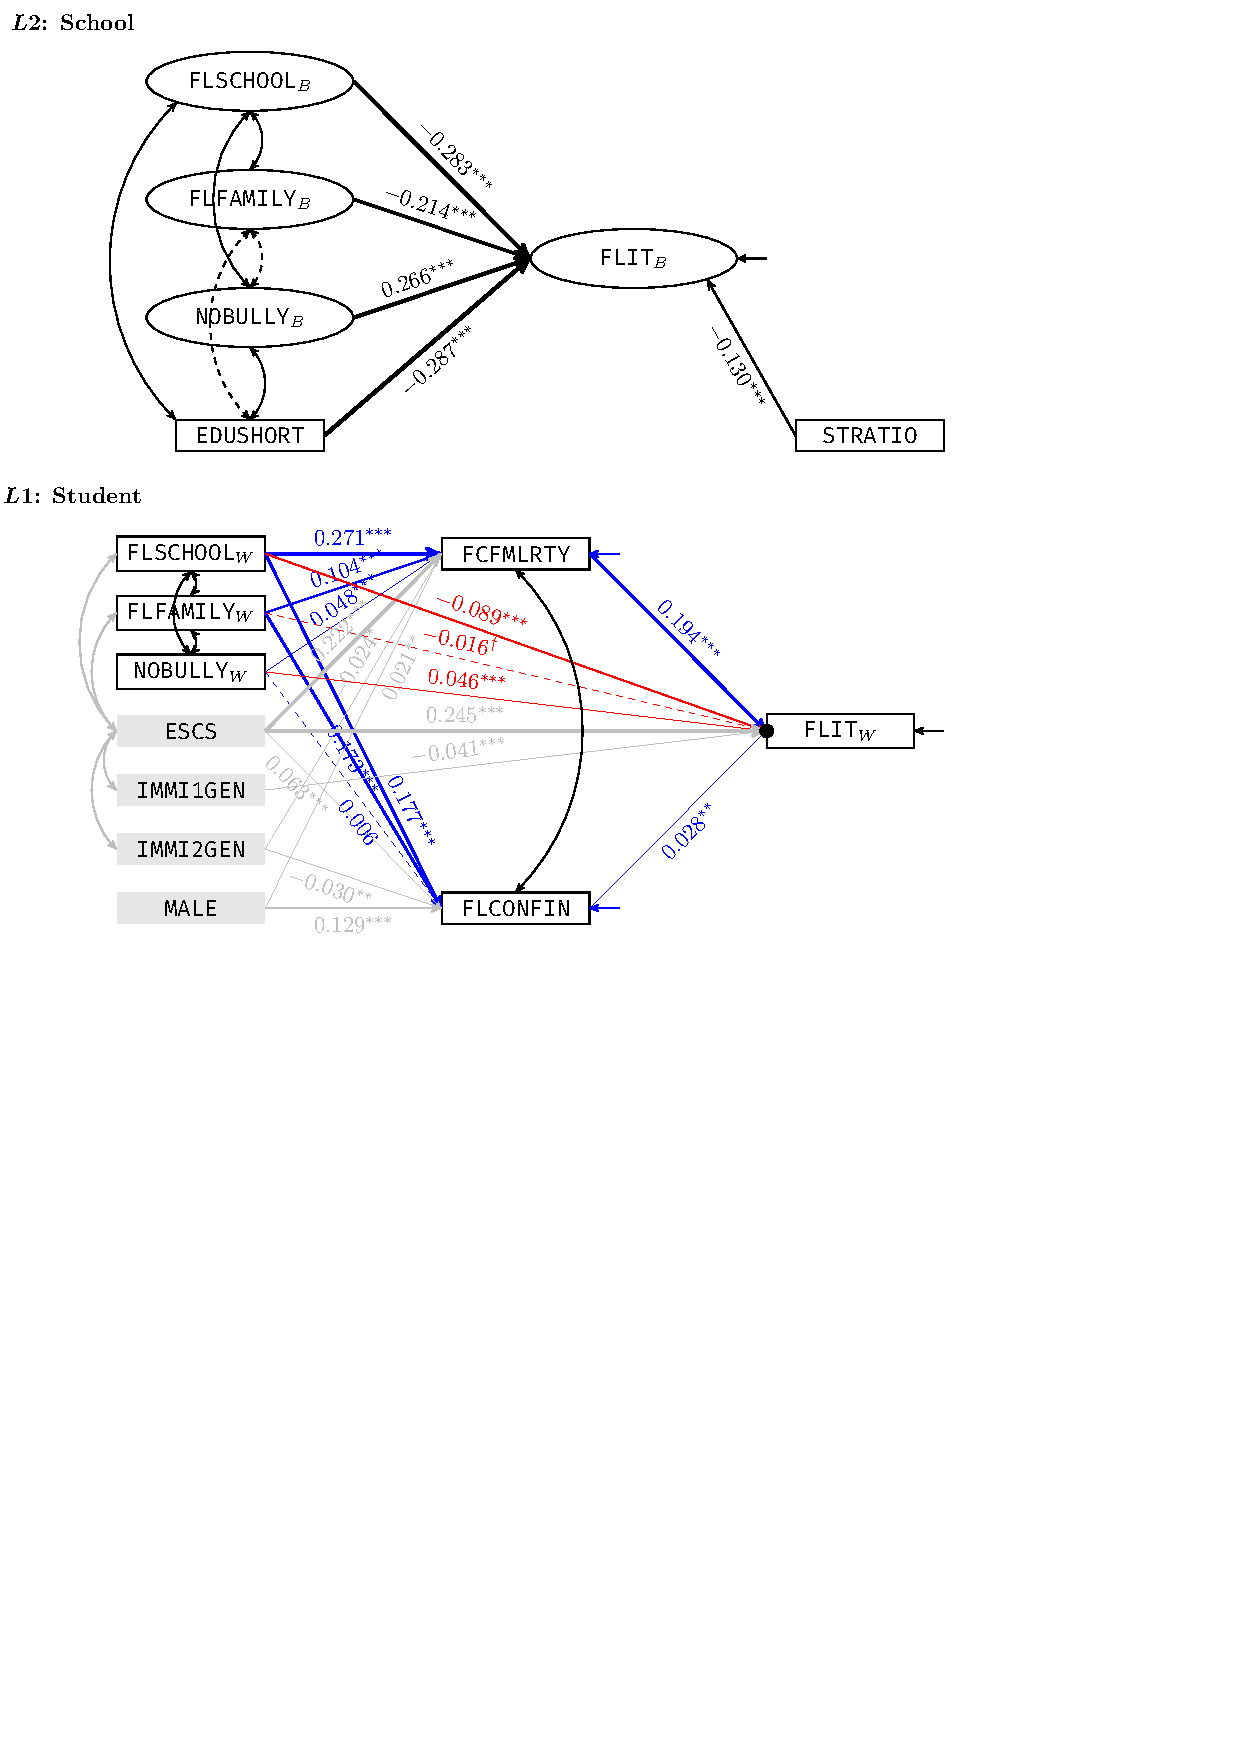
\includegraphics[width=0.9\textwidth]{../Figures/Poster_result.pdf}
        \end{figure}
    \end{block}

    \begin{block}{Conclusion}
        \begin{enumerate}
            \item[RQ1:] All four school climate variables significantly covary with students' financial literacy outcomes
            \item[RQ2:] Classroom activities correlate positively with financial literacy via affective pathways, but negatively via cognitive pathway
        \end{enumerate}
    \end{block}

    \begin{block}{References}
        \printbibliography
    \end{block}

\end{column}
% End right column

\end{columns}

% Bottom banner
\begin{textblock}{0.5}(0.18, 0.94)
    \color{white}
    \sffamily
    \textbf{Corresponding author}
    \\
    Tony Tan\ \ \url{tctan@uio.no}\\
    PO Box 1161, Blindern, 0318 OSLO, Norway
\end{textblock}

\end{frame}

\end{document}